\documentclass[tikz,border=2pt]{standalone}
\usepackage{amsmath,amssymb}
\usepackage{tikz}
\usetikzlibrary{arrows.meta}

\begin{document}
% Conjugation reflects z in the real axis: same modulus, opposite argument.
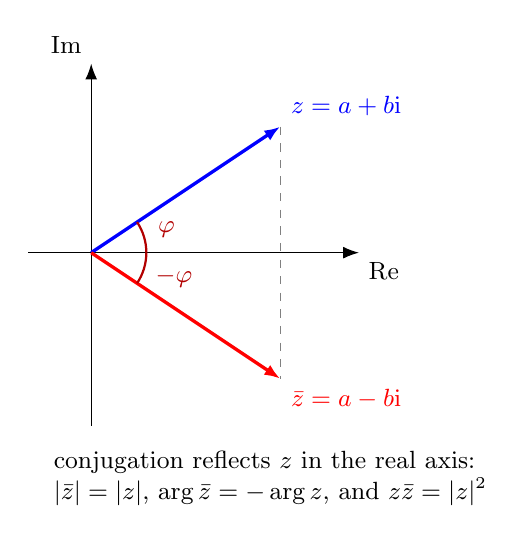
\begin{tikzpicture}[every node/.style={font=\small}, >={Latex[length=2mm]}]
	\draw[->] (-0.8,0) -- (3.4,0) node[below right] {$\mathrm{Re}$};
	\draw[->] (0,-2.2) -- (0,2.4) node[above left] {$\mathrm{Im}$};
	\draw[->, blue, very thick] (0,0) -- (2.4,1.6) node[above right] {$z=a+b\mathrm{i}$};
	\draw[->, red, very thick] (0,0) -- (2.4,-1.6) node[below right] {$\bar z=a-b\mathrm{i}$};
	\draw[dashed, gray] (2.4,1.6) -- (2.4,-1.6);
	\draw[red!70!black, thick] (0.7,0) arc (0:33.7:0.7);
	\node[red!70!black, font=\small] at (17:1.0) {$\varphi$};
	\draw[red!70!black, thick] (0.7,0) arc (0:-33.7:0.7);
	\node[red!70!black, font=\small] at (-17:1.1) {$-\varphi$};
	\node[anchor=north west, align=left] at (-0.6,-2.4) {conjugation reflects $z$ in the real axis:\\ $|\bar z|=|z|$, $\arg\bar z=-\arg z$, and $z\bar z=|z|^2$};
\end{tikzpicture}
\end{document}
